% Template file for an a0 landscape poster.
% Written by Graeme, 2001-03 based on Norman's original microlensing
% poster.
%
% See discussion and documentation at
% <http://www.astro.gla.ac.uk/users/norman/docs/posters/> 
%
% $Id: poster-template-landscape.tex,v 1.2 2002/12/03 11:25:46 norman Exp $


% Default mode is landscape, which is what we want, however dvips and
% a0poster do not quite do the right thing, so we end up with text in
% landscape style (wide and short) down a portrait page (narrow and
% long). Printing this onto the a0 printer chops the right hand edge.
% However, 'psnup' can save the day, reorienting the text so that the
% poster prints lengthways down an a0 portrait bounding box.
%
% 'psnup -w85cm -h119cm -f poster_from_dvips.ps poster_in_landscape.ps'

\documentclass[a0]{a0poster}
% You might find the 'draft' option to a0 poster useful if you have
% lots of graphics, because they can take some time to process and
% display. (\documentclass[a0,draft]{a0poster})
\input defs
\pagestyle{empty}
\setcounter{secnumdepth}{0}
\renewcommand{\familydefault}{\sfdefault}
\newcommand{\QED}{~~\rule[-1pt]{8pt}{8pt}}\def\qed{\QED}

\renewcommand{\reals}{{\mbox{\bf R}}}

% The textpos package is necessary to position textblocks at arbitary 
% places on the page.
\usepackage[absolute]{textpos}

\usepackage{fleqn,psfrag,wrapfig,tikz}

\usepackage{amsmath,amsfonts,amssymb,amsthm,mathtools} 
\usepackage[boxed]{algorithm2e}% http://ctan.org/pkg/algorithm2e
\makeatletter
\renewcommand{\@algocf@capt@plain}{above}% formerly {bottom}
\makeatother
\usepackage{algorithmic} 
\usepackage[papersize={38in,28in}]{geometry}

% Graphics to include graphics. Times is nice on posters, but you
% might want to switch it off and go for CMR fonts.
\usepackage{graphics}


% we are running pdflatex, so convert .eps files to .pdf
%\usepackage[pdftex]{graphicx}
%\usepackage{epstopdf}

% These colours are tried and tested for titles and headers. Don't
% over use color!
\usepackage{color}
\definecolor{Red}{rgb}{0.9,0.0,0.1}

\definecolor{bluegray}{rgb}{0.15,0.20,0.40}
\definecolor{bluegraylight}{rgb}{0.35,0.40,0.60}
\definecolor{gray}{rgb}{0.3,0.3,0.3}
\definecolor{lightgray}{rgb}{0.7,0.7,0.7}
\definecolor{darkblue}{rgb}{0.2,0.2,1.0}
\definecolor{darkgreen}{rgb}{0.0,0.5,0.3}

\renewcommand{\labelitemi}{\textcolor{bluegray}\textbullet}
\renewcommand{\labelitemii}{\textcolor{bluegray}{--}}

\setlength{\labelsep}{0.5em}


% see documentation for a0poster class for the size options here
\let\Textsize\normalsize
%\def\Head#1{\noindent\hbox to \hsize{\hfil{\LARGE\color{bluegray} #1}}\bigskip}
\def\Head#1{\noindent{\LARGE\color{bluegray} #1}\bigskip}
\def\LHead#1{\noindent{\LARGE\color{bluegray} #1}\bigskip}
\def\Subhead#1{\noindent{\large\color{bluegray} #1}\bigskip}
\def\Title#1{\noindent{\VeryHuge\color{Red} #1}}


% Set up the grid
%
% Note that [40mm,40mm] is the margin round the edge of the page --
% it is _not_ the grid size. That is always defined as 
% PAGE_WIDTH/HGRID and PAGE_HEIGHT/VGRID. In this case we use
% 23 x 12. This gives us three columns of width 7 boxes, with a gap of
% width 1 in between them. 12 vertical boxes is a good number to work
% with.
%
% Note however that texblocks can be positioned fractionally as well,
% so really any convenient grid size can be used.
%
\TPGrid[40mm,40mm]{23}{12}      % 3 cols of width 7, plus 2 gaps width 1

\parindent=0pt
\parskip=0.2\baselineskip

\definecolor{mygray}{gray}{0.6}
\begin{document}

% Understanding textblocks is the key to being able to do a poster in
% LaTeX. In
%
%    \begin{textblock}{wid}(x,y)
%    ...
%    \end{textblock}
%
% the first argument gives the block width in units of the grid
% cells specified above in \TPGrid; the second gives the (x,y)
% position on the grid, with the y axis pointing down.

% You will have to do a lot of previewing to get everything in the 
% right place.

% This gives good title positioning for a portrait poster.
% Watch out for hyphenation in titles - LaTeX will do it
% but it looks awful.
\begin{textblock}{23}(0,0)
\Title{Q-Learning: randomized rewards}
\end{textblock}

\begin{textblock}{23}(0,0.6)
{
\LARGE
Valentin Samokhin, Daniil Merkulov
}

{
\Large
\color{bluegray}
\emph{Optimization Class Project. MIPT}
}
\end{textblock}


% Uni logo in the top right corner. A&A in the bottom left. Gives a
% good visual balance, but you may want to change this depending upon
% the graphics that are in your poster.
%\begin{textblock}{2}(0,10)
%Your logo here
%%\includegraphics{/usr/local/share/images/AandA.epsf}
%\end{textblock}

%\begin{textblock}{2}(21.2,0)
%Another logo here
%%\resizebox{2\TPHorizModule}{!}{\includegraphics{/usr/local/share/images/GUVIu/GUVIu.eps}}
%\end{textblock}


\begin{textblock}{7.0}(0,1.5)

\hrule\medskip
\Head{Introduction}\\
The Reinforcement Learning (RL) is a quite old branch of learning based on interaction between the environment and the agent. The agent makes actions, receives reward, and makes a step according to some policy. The task of the RL is to find out the optimal policy that provides the biggest cumulative reward. There are two main approaches in RL - model-based and model-free. The latter one is considered by some specialists to be more simple in sense of memory consumption and knowledge about the environment. Moreover, model-free approaches are suitable for on-line learning. The most difficult problems that algorithms should solve is the exploitation-exploration trade-off and the credit assignment problem. Instead of introducing arbitrariness into action choice we add Gaussian noise to the reward received by the agent. Thus we want to study the possible effect the noise can bring into the results. To our disappointment, the majority of existing papers are not supported by any numerical experiments. We want to set them.

\medskip
\hrule\medskip
\Head{Value (V-) and action-value (Q-) functions}\\

Let us intrduce \textit{the Value function}:
\begin{equation}\label{eq::V_func}
V^\pi(s) = \mathbb{E}\left[\sum_i \gamma^i r_i(s_i, a^\pi_i)\mid s_0 = s, \pi \right]
\end{equation}
It is the expectation of the sum of discounted rewards, received by the agents in case it follows the policy $\pi$ \footnote{Policy is a function that maps from states to actions} starting from the state $s$.

Then we should introduce \textit{the Q-function}. It, given the state $s$ and action $a$, returns the expected cumulative reward in case of folowing the policy $\pi$
\begin{multline}\label{eq::Q_func}
Q^\pi (s, a) = \mathbb{E} \left[ \sum_{t\geq 0} \gamma^t r_t \mid s_0 = s, a_0 = a, \pi\right] =\\= r_0(s, a) + \gamma\mathbb{E} \left[V^\pi(s_1\footnote{$s_1$ might be sampled from some distribution},  a)\right]
\end{multline}
It makes sence, if we suppose that interaction between agent and environment is a Markov Decision Process. This assumption allows us not to take into the account the previous observations.

\textit{Optimality theorem} states that for the optimal policy $\pi^\star$ the following equation takes place.

\begin{equation}
V^\star  = max _a Q^\star(s,a)
\end{equation}

If we assume that the state and action spaces, and the horizon, than we can claim that the optimal policy always exists.
This equation and the recursive definition of Q-function \eqref{eq::Q_func} make possible the introduction of the various iterative schemes (like \eqref{eq::iteration})that update the Q-values step-by-step.
\begin{equation}\label{eq::iteration}
Q_{i+1}(s, a) = \mathbb{E}\left[r + \gamma max_{a^{'}} Q_i(s', a') \mid s, a\right]
\end{equation}


\end{textblock}

\begin{textblock}{7.0}(8,1.5)
\medskip
\hrule\medskip
\Head{Algorithm}\\
The main algorithm we want to study here is a variant of Q-learning that incorporates UCB exploration.
% чета не работает ((((((((
\begin{algorithm}[h!]
	\SetAlgoLined

	\label{UCBalg}
	\begin{algorithmic}[1]
		\STATE Initialize $Q_h(s, a) \leftarrow H$ and  $N_h(s, a)\leftarrow 0$ $\forall (s, a, h) \in S \times A \times \left[H\right] $
		\FOR {episode $k=1,.., K$}
		\STATE Receive $x_1$
		\FOR {step $h = 1, \dots, H$ }
		\STATE {Take action $a_h \leftarrow \argmax_{a'} Q_h(x_h, a')$, and observe $x_{h+1}$}
		\STATE $t=N_h(s_h,a_h)\leftarrow N_h(s_h,a_h)+1; b_t \leftarrow c\sqrt{H^3\iota /t}$
		\STATE $Q_h(s_h, a_h) \leftarrow (1 - \alpha_t)Q_h(s_h, a_h) + \alpha_t[r_h(s_h, a_h) + \mathcal{N}(0,1)+ V_{h+1}(s_{h+1}) + b_t]$. $V_h(s_h) \leftarrow min\{H, \max_{a^{'}\in A} Q_h(s_h, a^{'})\}$.
		\ENDFOR
		\ENDFOR
	\end{algorithmic}
	\caption{Q-learning with UCB-Hoeffding}
\end{algorithm}

Here $\iota$ is a log-factor: $\iota := \log(SAT/p)$


We would compare this approach with $\epsilon$-greedy policy without bonus: instead of choosing the best action from the Q-table (as in step 5 of the algorithm \ref{UCBalg}), we would balance between exploitation and exploration with $\epsilon$ probability of choosing exploration. We would also try to add some small noise to the reward in the UCB-algorithm (step 7).


\begin{algorithm}[h!]
	\SetAlgoLined
	
	\label{UCBalg}
	\begin{algorithmic}[1]
		\STATE Initialize $Q_h(s, a) \leftarrow H$ and  $N_h(s, a)\leftarrow 0$ $\forall (s, a, h) \in S \times A \times \left[H\right] $
		\FOR {episode $k=1,.., K$}
		\STATE Receive $x_1$
		\FOR {step $h = 1, \dots, H$ }
		\STATE {Sample action $a_h \leftarrow \argmax_{a'} Q_h(x_h, a')$ with $p = 1-\epsilon$ or chose any other action with $p=\epsilon$, and observe $x_{h+1}$}
		\STATE $t=N_h(s_h,a_h)\leftarrow N_h(s_h,a_h)+1; b_t \leftarrow c\sqrt{H^3\iota /t}$
		\STATE $Q_h(s_h, a_h) \leftarrow (1 - \alpha_t)Q_h(s_h, a_h) + \alpha_t[r_h(s_h, a_h) + V_{h+1}(s_{h+1}) + b_t]$. $V_h(s_h) \leftarrow min\{H, \max_{a^{'}\in A} Q_h(s_h, a^{'})\}$.
		\ENDFOR
		\ENDFOR
	\end{algorithmic}
	\caption{Q-learning with $\epsilon$-greedy exploration}
\end{algorithm}



\hrule\medskip
\Head{Numerical example}\\
To get numerical results we use the environment from Open-AI gym package "Taxi-v2". It has small finite action and observation spaces and allows user to select the arbitrary initial state. 
\begin{quotation}
	There are 4 locations (labeled by different letters) and your job is to pick up the passenger at one location and drop him off in another. You receive +20 points for a successful dropoff, and lose 1 point for every timestep it takes. There is also a 10 point penalty for illegal pick-up and drop-off actions.
\end{quotation}

\end{textblock}

\begin{textblock}{7.0}(16,1.5)
\medskip
\hrule\medskip
\Head{Results}\\
The results show, that UCB-exploration finds the optimal policy quicker than the $\epsilon$-greedy algorithm. The addition of noise makes the curve of the episode reward smoother for both policies. 
\begin{center}

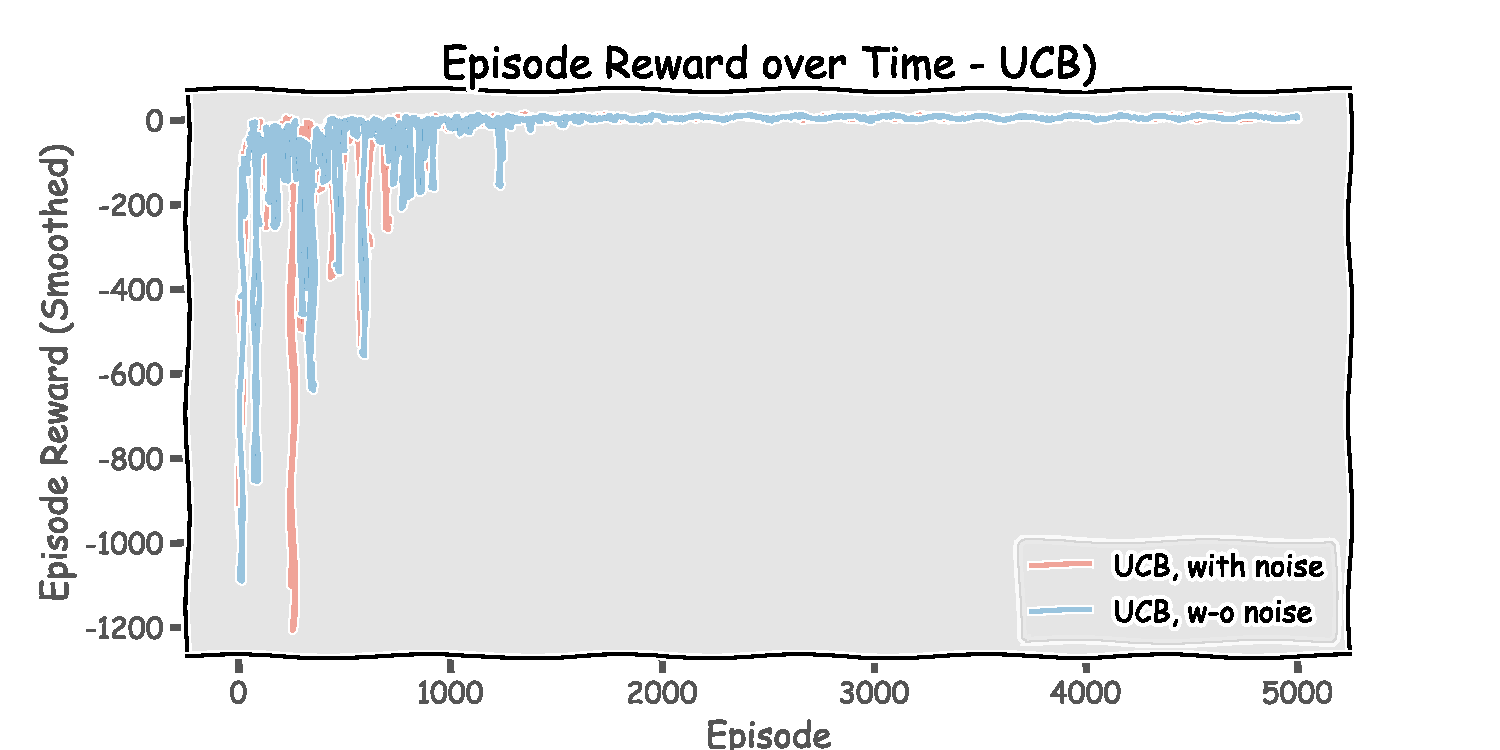
\includegraphics[width=0.9\textwidth]{figures/UCB.pdf}
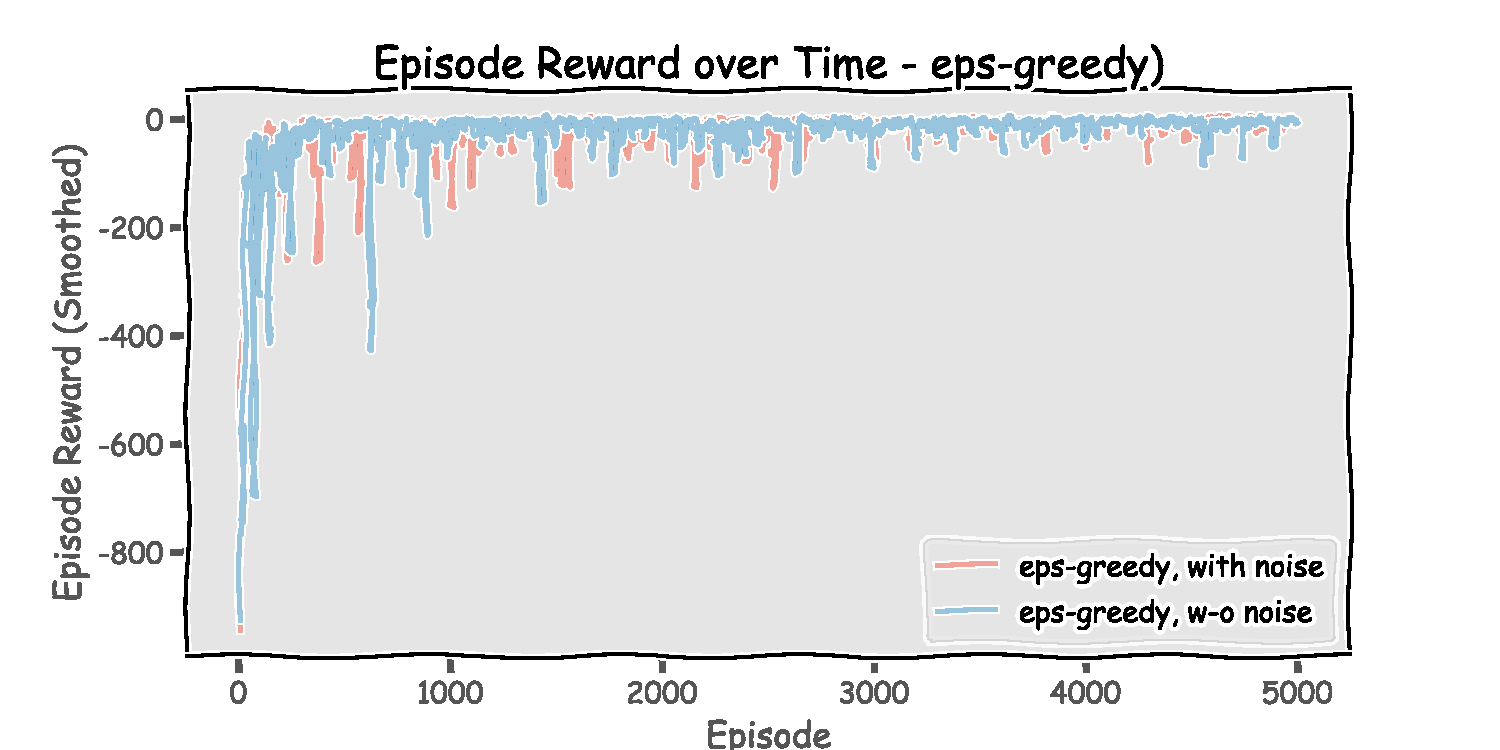
\includegraphics[width=0.9\textwidth]{figures/eps-greedy.pdf}
\end{center}

\medskip
\hrule\medskip
\Head{Conclusion}\\
We showed that in some cases bonus and noise addition may help to improve the exploration-exploitation trade-off, giving better observed episode rewards. 


\medskip
\hrule\medskip
\Head{Acknowledgements}\\
This material is based upon work supported by the unequal contribution of different activities to the final mark for the optimization course.
\textcolor{mygray}{
\medskip
\hrule\medskip
\Head{\textcolor{mygray}{Comments}}\\
	What I am goind to improve in my work is:
	\begin{itemize}
		\item[\textcolor{mygray}{$\bullet$}] code: more accurate
		\item[\textcolor{mygray}{$\bullet$}]  grid search for some parameters (constant in the bonus definition)
		\item[\textcolor{mygray}{$\bullet$}]  more methods
		\item[\textcolor{mygray}{$\bullet$}]  theoratical support
		\item[\textcolor{mygray}{$\bullet$}]  citations
	\end{itemize}
}
\end{textblock}

\end{document}